\chapter{Конструкторский раздел}

В данном разделе будут спроектированы схемы алгоритмов, описаны используемые типы данных, а также произведена оценка памяти и описана структура ПО.

\section{Схемы алгоритмов}

На рисунках 2.1 - 2.3 представлены схемы рассматриваемых алгоритмов.

\begin{figure}[h!]
	\begin{center}
		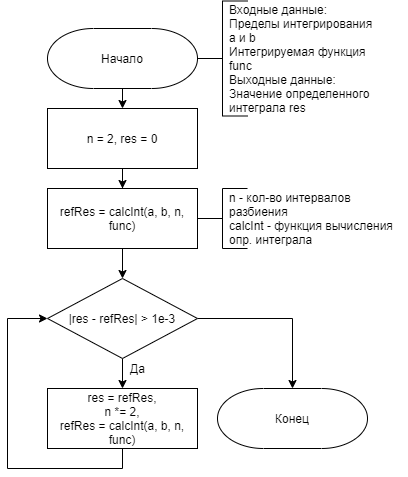
\includegraphics[scale=0.7]{assets/refineIntegral.png}
	\end{center}
	\caption{Схема алгоритма последовательного вычисления значения определенного интеграла}
\end{figure}

В данном алгоритме используется функция вычисления определенного интеграла (рисунок 2.2).

\newpage 
\begin{figure}[h!]
	\begin{center}
		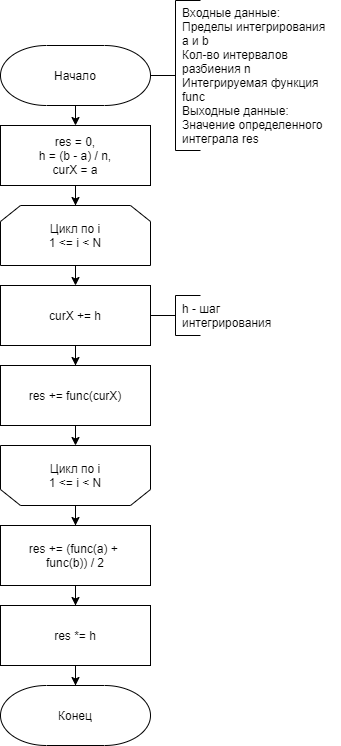
\includegraphics[scale=0.7]{assets/calculateIntegral.png}
	\end{center}
	\caption{Схема алгоритма вычисления значения определенного интеграла}
\end{figure}

\newpage 
\begin{figure}[h!]
	\begin{center}
		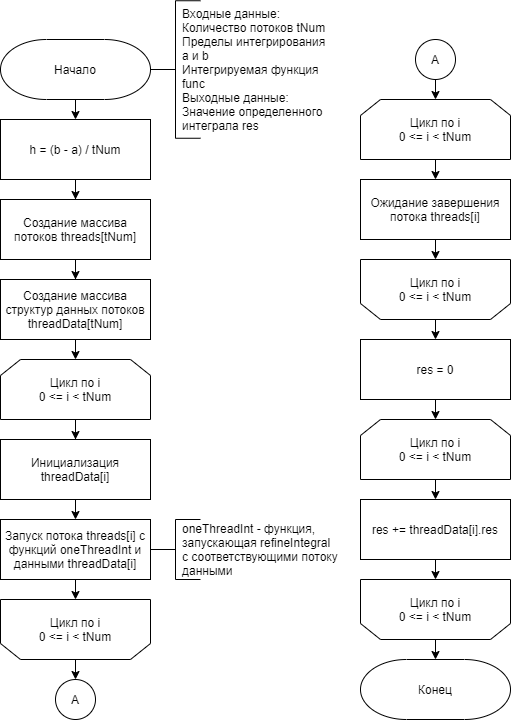
\includegraphics[scale=0.7]{assets/integralThreads.png}
	\end{center}
	\caption{Схема алгоритма параллельного вычисления значения определенного интеграла}
\end{figure}

\newpage
\section{Используемые типы данных}

При реализации алгоритмов будут использованы следующие структуры данных:
\begin{itemize}
	\item границы интервалов интегрирования, аргументы и значения функций - вещественные числа double;
	\item потоки - массив типа pthread\_t;
	\item данные потоков - массив типа threadData. 
\end{itemize}

Тип threadData описан в листинге ниже.

\captionsetup{singlelinecheck = false, justification=raggedright}
\begin{lstlisting}[label=threadData, caption=Тип данных потока]
typedef double(*integralFunc)(double);

struct threadData{
    int ind;
    double a;
    double h;
    integralFunc func;
    double res;
};
\end{lstlisting}
\captionsetup{singlelinecheck = false, justification=centering}

\section{Оценка памяти}

Рассмотрим затрачиваемый объем памяти для рассмотренных алгоритмов. 

При последовательном вычислении память используется на:
\begin{itemize}
	\item входные параметры функции - 2 * sizeof(double) + sizeof(double *);
	\item возвращаемое значение - sizeof(double);
	\item вспомогательные переменные - sizeof(int) + sizeof(double);
	\item память, используемая функцией calcInt, а именно:
	\begin{itemize}
		\item входные параметры функции - 2 * sizeof(double) + sizeof(int) + sizeof(double *);
		\item возвращаемое значение - sizeof(double);
		\item вспомогательные переменные - 3 * sizeof(double).
	\end{itemize}
\end{itemize}

В случае параллельного вычисления для каждого потока помимо описанной выше используемой памяти выделяется структура threadData, размер которой равен sizeof(double) + sizeof(int) + sizeof(double *).
Также внутри функции, создающей потоки выделяется память:
\begin{itemize}
	\item возвращаемое значение - sizeof(double);
	\item массив потоков - $tNum$ * sizeof($pthread\_t$);
	\item вспомогательные переменные - 2 * sizeof(double).
\end{itemize}

Таким образом, для параллельного вычисления используется в $tNum$ раз больше памяти, где $tNum$ - количество потоков.

\section{Структура ПО}

ПО будет состоять из следующих модулей:
\begin{itemize}
	\item главный модуль - из него будет осуществляться запуск программы и выбор соответствующего режима работы;
	\item модуль интерфейса - в нем будет описана реализация режимов работы программы;
	\item модуль, содержащий реализации алгоритмов.
\end{itemize}

\section{Вывод}

На основе полученных в аналитическом разделе знаний об алгоритмах были спроектированы схемы алгоритмов, выбраны используемые типы данных, проведена оценка затрачиваемого объема памяти, а также описана структура ПО.